%%%%%%%%%%%%%%%%%%%%%%%%%%%%
% DOCUMENT SETUP & IMPORTS
%%%%%%%%%%%%%%%%%%%%%%%%%%%%
\documentclass[10pt,letterpaper,oneside,english]{article}
\usepackage[margin=.5in]{geometry}
\usepackage[utf8]{inputenc}
\usepackage{setspace}
	\onehalfspace

\usepackage{enumerate}
\usepackage{graphicx}
\usepackage{hyperref}
\usepackage{xcolor}

% \usepackage{enumitem}
% 	\setenumerate[1]{label=\textit{\arabic*}}
% 	\setenumerate[2]{label=\textbf{\alph*},topsep=0pt}

%%%%%%%%%%%%%%%%%%%%%%%%%%%%
% USER-DEFINED COMMANDS
%%%%%%%%%%%%%%%%%%%%%%%%%%%%
% Usage: \person{<last>}{<first>}{<email>}
\newcommand{\person}[3]{
	#1, #2\\
	\href{mailto:#3}{\texttt{#3}}
}
\newcommand{\ncomp}{\emph{non-complete}}


\newcommand{\prog}{\emph{in progress}}

\newcommand{\see}[1]{(see {\color{blue!60!black}\nameref{#1}})}

\newcommand{\chref}[2]{\href{#1}{{\color{blue!60!black}#2}}}

\newcommand{\wref}{\href{http://en.wikipedia.org/wiki/Main_Page}{({\color{blue!60!black}from Wikipedia})}}

\newcommand{\solution}{\newline \hspace*{1em} \textbf{Solution: }}

\newcommand{\code}[1]{\texttt{#1}}

\newcommand{\citem}[1]{\item \code{#1}}

\newcommand{\gls}[2]{ \ \\ \hspace*{1em} \textbf{#1} \ \\ \hspace*{1.5em}{#2}}


%%%%%%%%%%%%%%%%%%%%%%%%%%%%
% TITLE AUTHORS AND DATE
%%%%%%%%%%%%%%%%%%%%%%%%%%%%
\title{
	\textbf{Game Engine Development Team}\\
	Final Report v1.0
}

\author{
	\person{Bahr}{Dan}{dbahr92@gmail.com}
	\and
	\person{Bard}{Etan}{ebard@ups.edu}
	\and
	\person{Burns}{Nick}{nbburns@ups.edu}
	\and
	\person{Livingston}{Chris}{christopherlivingston92@gmail.com}
	\and
	\person{Wilson}{Robin}{rkwilson@ups.edu}
}
\date{\today}



%%%%%%%%%%%%%%%%%%%%%%%%%%%%
% DOCUMENT
%%%%%%%%%%%%%%%%%%%%%%%%%%%%
\begin{document}
\maketitle
\newpage

\tableofcontents
\newpage

\section{Cover Page}

\section{Abstract}
The game development group is creating a stand-alone survival/platform game, which will also be capable of taking inputs from a Kinect and mobile phones. Once completed, this project will provide a simple to learn, hard to master style of play, in which players will compete against people using mobile phones.\\
This document describes the final and complete state of the game. Outlined within are summaries of the requirements for the game as well as the design thereof, complete within diagrams and a complete implementation description. Finally, this document describes our testing methodology and a reflection of the overall process and participation in this project.

\section{Functional Requirements}

\subsection{Main Use Case}
\subsubsection{Actors} Server, Kinect, Display, Mobile Devices(phones), Game Computer, Puppeteers (Jump, Movement, SpecialMovement, Item-use)
\subsubsection{Preconditions} The Kinect works on the game computer and can read actions of the puppeteers. The puppeteers know which action corresponds to their role. The augmented reality system can identify objects. The network is avalible and functioning with low lag
\subsubsection{Postconditions} The game computer, along with the phones, and server are functional. The score has been displayed and logged.
\subsubsection{Main Scenario}
\begin{enumerate}
\item \textbf{The Game Computer starts game engine.} \\ At this point, the vast majority of the game initialization will be done by the Unity engine. All images and meshes, for example, will be preloaded (but this is all invisible to the user).
\item \textbf{The Game Computer contacts the Server.} \\ This will we done with a request for connection with a predetermined protocol. This connection will be used for the remainder of the gaming session (until termination for any reason).
\item \textbf{The game computer connects to the Kinect.} \\ This step involves any initialization required for establishing and maintaining a connection similar to the connection made with the server.
\item \textbf{The game engine displays the main menu.} \\ This will include options for the puppeteers to pick their roles.
\item \textbf{The game engine displays instructions, to the user.} \\ English language visual instructions will direct players to start the game. Puppeteers will be prompted with instructions on how to choose their roles.
\item \textbf{The puppeteers motion to start the game.} \\ We will receive a command from the Kinect notifying that the game is to start. Visually, this will be where the game appears to begin.
\item \textbf{The computer gets augmented reality data from the phones.} \\ The locations of augmented reality objects will be detected by the augmented reality group and relayed to the game engine through the web server.
\item \textbf{The game engine creates the world using the data collected from the augmented reality group about the real-world environment.} \\ Codes from the augmented reality group will be placemarks for 3D models in the rendered world. These could be buildings, platforms, enemy spawners, etc.
\item \textbf{While game continues, the following will occur.}
	\begin{enumerate}
\item \textbf{The actions of the player are used to modify the game state.} \\ For example, when we get a command from the Kinect to move forward, the character on screen will do the appropriate action. Player actions can occur at any time.
\item \textbf{Augmented Reality and other dynamic data is sent from the phones to the game engine.} \\ For example, we may receive a command from the server to place an object in a certain location for the character to interact with.
\item \textbf{The game state is updated and tracked.} \\ Any necessary updating is finished before rendering.
\item \textbf{The game engine renders the world.} \\ This is all handled by Unity automatically. The game will be displayed on a screen.
\item \textbf{The world data is sent to the phones.} \\ Character data, obstacle data, and so forth may all be sent to the server to forward on the phones for rendering.
\end{enumerate}
\item \textbf{The game completes.} \\ The game is finished when a certain victory condition or loss condition is achieved (for example, if the character dies).
\item \textbf{The game’s statistics are displayed                                                                                                                                                                                                   .} \\ Details about the puppeteer’s performance, such as overall score, time until imminent death, enemies killed, in-game accomplishments, etc. are displayed on the screen.
\item \textbf{The server logs the game’s score.} \\ We send the score data to the server.
\item \textbf{Return to the main menu.} \\ Here the users can choose to play again (going back to step 4) or quit the game.
\item \textbf{A player selects the quit option.}
\item \textbf{All network connections are terminated.} \\ The connections to the server and the Kinect will both be shut down, forcefully if need be.
\item \textbf{The game engine shuts down.} \\ This is handled by Unity. It will clean up any resources used by the game engine and exit the application.
\end{enumerate}

\subsubsection{Alternative Scenarios}
\begin{description}
\item[1-4] Unity fails to load properly.
\solution{May be resolved by computer restart or simply restarting Unity3D. At this point, there’s not much we can do, as Unity is supposed to handle all game initialization automatically without any user control.}
\item[5-6] If there is a failure to accurately display main menu.
\solution{Correct the video settings. It is possible that the computer’s graphics settings are not configured correctly. This is the burden of the user to fix.}
\solution{Restart the game. Again, this is probably Unity’s fault.}
\item[any] low frame rate, lag
\solution{Reduce the number of displayed objects, reduce textures, reduce anti-aliasing. There are a number of tricks we can do to reduce the number of objects on screen to alleviate this problem.}
\solution{Provide a mechanism for changing graphics settings to improve performance.}
\item[5-20] There are networking problems.
\solution{Check to make sure that all network communications are available. Perform checks on the connection to the server and allow the user to try to reconnect.}
\item[any] If the game fails to respond.
		\solution{Restart the game. Sorry game users! Let’s just hope it never gets to this point \textellipsis}

\end{description}



\section{Non-Functional Requirements}

\subsection{Usability}
\begin{enumerate}
\item \textbf{Interface is Easily Navigable} The Puppeteers can navigate menus displayed on the main projector, and are able to choose options that they want. Players are able to choose buttons using the Kinect or use the phones. We can tell we accomplished this from Puppeteers feedback.
\item \textbf{Legibility of Textual Feedback} Puppeteers must be able to read text written on the projector from across the room, and mobile users can read text on Mobile Devices from a distance of at least one meter. (Puppeteers feedback)
\item \textbf{Replay Value} The game should be fun to play, and provide challenging gameplay no matter the skill level. Players should be compelled either by the story, the gameplay, or interaction with the other players. We can tell if we achieved this through Puppeteers and Mobile Device operators feedback. If 85\% of our players (Puppeteers and Mobile Device operators are enjoying themselves then we’ve done our part).
\end{enumerate}
\subsection{Reliability}
\begin{enumerate}
\item \textbf{Stand-Alone Nature of Game Engine} \\ If the internet or the connections with the Mobile Devices, augmented reality, or Server get interrupted, gameplay should be able to continue through Kinect input.
\end{enumerate}
\subsection{Performance requirements}
\begin{enumerate}
\item \textbf{Fluidity of Gameplay} \\ The game should run with little to no lag at a framerate of at least 20. The movements done by the Puppeteers should be able to register with the Kinect and the avatar should respond on the main display in the proper way in less than one second. All data sent between the   
\item \textbf{Ability to support a large number of generated objects.} \\
The gameplay and the length of time the game loads should not depend on only a few objects being generated.

\item \textbf{The game is playable.} \\ The kinect needs to pick up the movements and display them quickly, the enemies on screen should die when the character kills them, the character animations should work according to the motions of the players.

\item \textbf{The kinect identifies movements in a timely manner.} \\ From when the Puppeteers do a physical movement on the Kinect the character should move accordingly inside the game and on the Display. It is possible the Motion Capture group will need to deal with this but we will have to take the input from the Kinect and make the character move.
\end{enumerate}
\subsection{Supportability}
\begin{enumerate}
\item \textbf{Windows 7 on the class’ server.} \\ Because we have machines that run Windows 7 we need to make an engine that works on Windows 7.

\end{enumerate}
\subsection{Implementation}
\begin{enumerate}
\item \textbf{The work is done in Unity3D.} \\ The customer would like us to work in Unity because it is a free application.
\item \textbf{C\# for coding.} \\ Unity uses C\#.
\end{enumerate}
\subsection{Environmental}
\begin{enumerate}
\item \textbf{Aesthetically pleasing} \\ The graphics should not look only like gray blocky graphic shapes. We would like there to be textures covering the skeletons of the boxes, enemies generated, and on the character. Although this is not necessary for the gameplay, the Game Design group would like to uphold this standard.
\end{enumerate}

\section{Architecture Design}
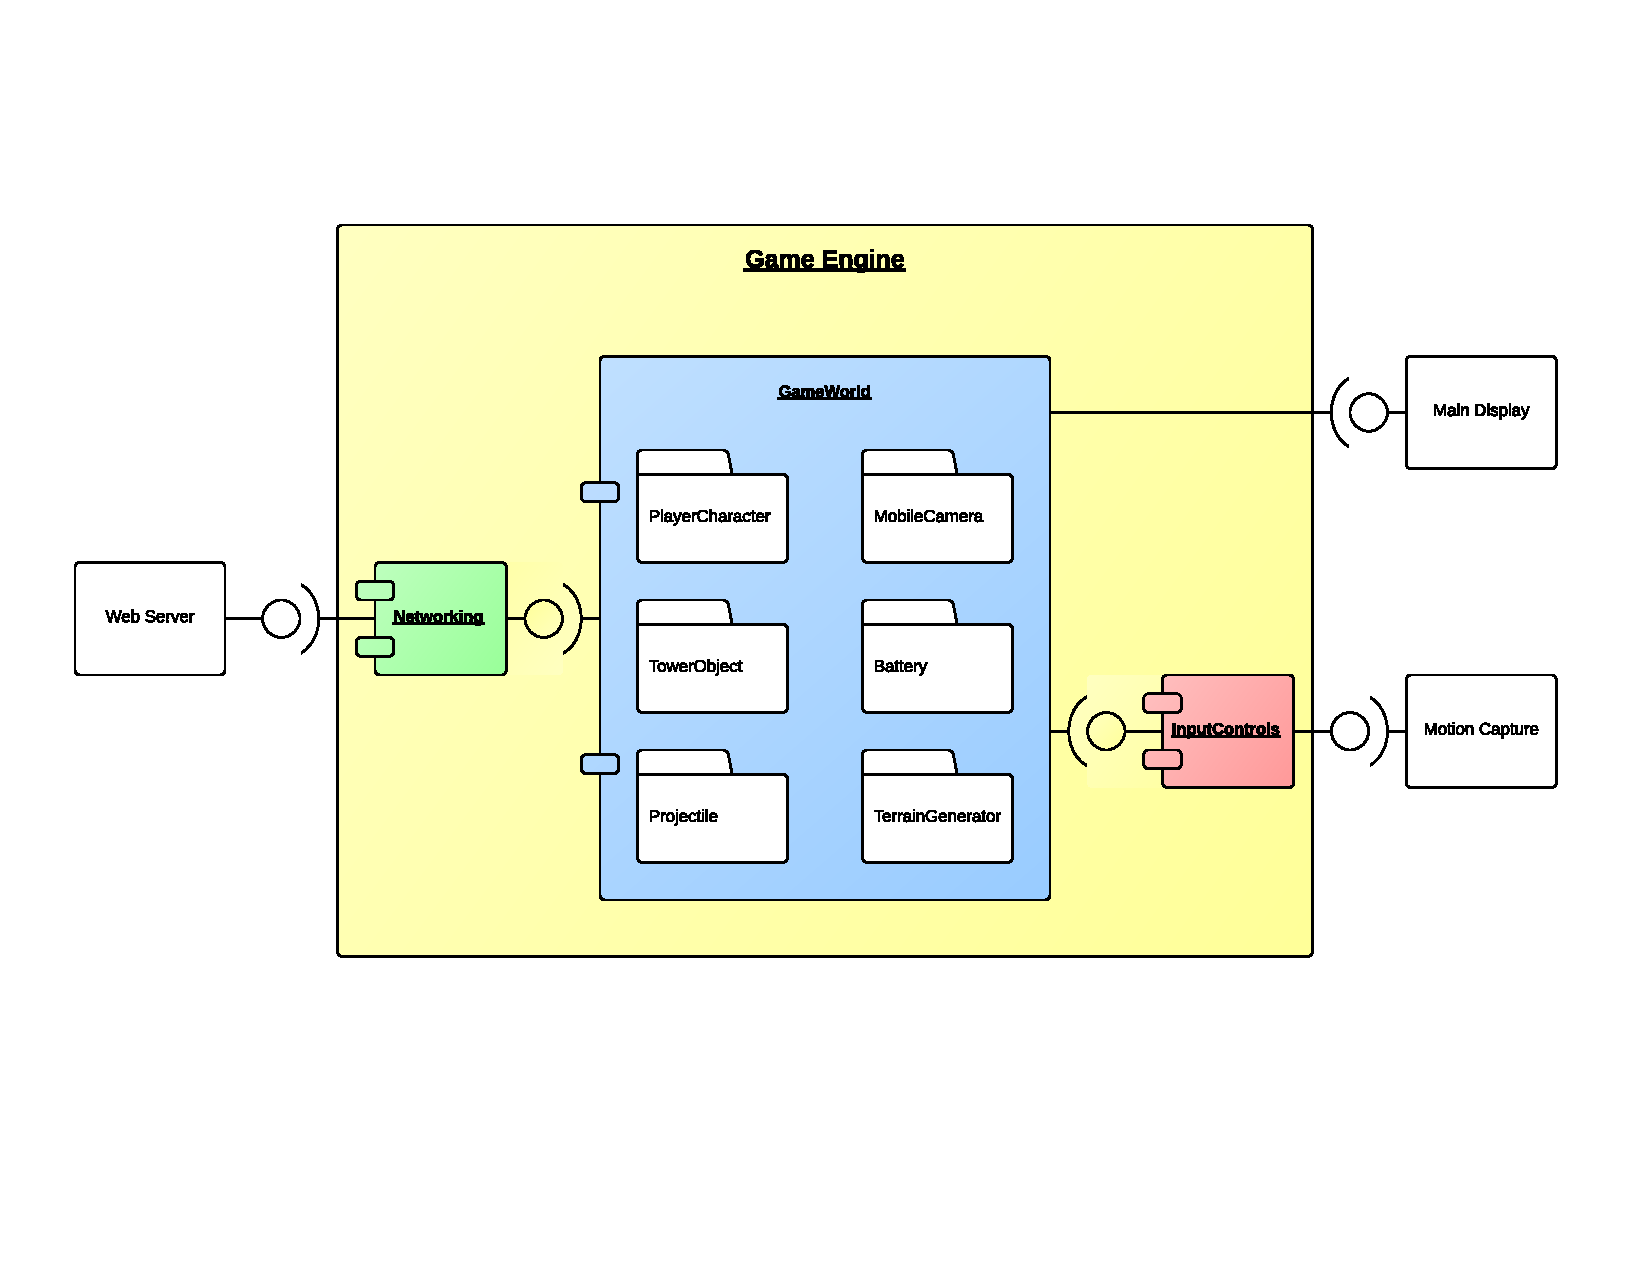
\includegraphics[scale=.6]{comp}\\
Three major modules exist: the GameWorld, InputControls, and Networking. The GameWorld includes several classes, each with a specific role which can typically be thought of as encapsulating a single object in the game, such as a battery that the character can collect, or a projectile that the character will attempt to dodge. GameWorld from a high-level standpoint monitors the state of all game objects, such as the state of the platforms and items. All of the information about
the game world itself is stored in this module. InputControls is the interface for the motion capture group, which is used for character actions. The Networking module interfaces with the web server, providing updates for the mobile devices in the GameWorld such as character data and scores. This module also receives real-time data from the mobile devices about augmented reality and other data.\\
The communication between the modules is simple: the Networking and GameWorld modules communicate with each other, and the InputControls and GameWorld modules communicate with each other. The Networking and InputControls modules will never communicate with each other directly; any state information is first directed through the GameWorld module for proper handling.

\section{Module Design}

\subsection{InputControls}

\subsubsection{Description}
The InputControls module contains individual functions for specific tasks (see Provided Interface). These functions will be called in order to move the character or have the character perform an action. Thus, the InputControls module is the interface between the character movements and the outside world.\\
This module is responsible for consolidating all of the actions that a character can perform. It will allow us to control the character from multiple inputs simultaneously and will be used primarily as an interface between the game engine and the motion capture.

\subsubsection{Provided Interface}
Functions for controlling the Character. Examples:
\begin{enumerate}
	\item void Jump(float magnitude);
	\item void MoveForward(float magnitude);
	\item void MoveBackward(float magnitude);
	\item void RotateLeft(float magnitude);
	\item void RotateRight(float magnitude);
	\item void Attack();
    \item void Shield();
\end{enumerate}

\subsubsection{Required Interface}
\begin{enumerate}
\item getKinectActions();
\end{enumerate}

\subsection{GameWorld}

\subsubsection{Description}
The game world is our main module. This module includes several classes which interact with each other to simulate the game world. For example, a minion might attack the character, and the character may pick up a shield power-up to protect itself. All of this interaction occurs in the GameWorld module.\\
The GameWorld module essentially keeps track of the static and dynamic objects and where exactly the character is in the world. The GameWorld is responsible for getting inputs from the InputControls Module for the character and getting inputs from the Network Module for where the augmented reality objects are. This module will also take care of rendering the game world and the background. Sound will also be maintained within the GameWorld. The GameWorld will optionally spawn items depending on what the Web Server group gets on twitter.

\subsubsection{Provided Interface}
\begin{enumerate}
	\item Character direction and position, object placement, enemy direction and placement.
 	\item Game-world display for MainDisplay    
\end{enumerate}

\subsubsection{Required Interface}
\begin{enumerate}
    \item Object creation and placement from Network Interface Module (Web Server group)
	\item Twitter inputs from Network Interface Module(Web Server Group)
	\item getActions() from InputControls Module
	\item getMobileDevicePosition() from Network Module (Server group)
\end{enumerate}

\subsection{Network}

\subsubsection{Description}
The Network module encapsulates everything concerning networked communications and speaking to the web server. It will provide functions for sending data in a clear manner with a well-defined API that can be used from within the other functions. It will automatically send character data and object data from the GameWorld module. It will provide an interface for receiving data from the server as well (such as data about new augmented reality objects).

\subsubsection{Provided Interface}
Functions for sending data to the web server via HTTP requests and a JSON object.
\begin{enumerate}
\item void SendUpdatedJSONData();	
\end{enumerate}

\subsubsection{Required Interface}
	Functions for retrieving character, object, and other game state data (as provided to this module by the GameWorld module).

\section{Implementation Description}

\subsection{Source Code Location}
Source code is hosted by \chref{https://github.com}{GitHub}. The repository for downloading the source code is located at the \chref{https://github.com/UPS-CS240-F12/main_trunk.git}{\texttt{main\_trunk}}. The develop branch is used by project developers and is guaranteed to contain the latest code (but which may or may not be stable). The master branch contains the latest stable release version.
\subsection{Installation Instructions}
In order to install and run the source code for the project, a develop must first download and install the \chref{http://unity3d.com/unity/download/}{Unity3D} game engine, and \chref{http://www.blender.org/download/get-blender/}{Blender}. To open up the Unity editor with the project, simply open up one of the .unity files contained in the /Game\_Engine/Assets/ folder of the repository. The entire project can be modified from within the Unity editor. Double-clicking on a script asset will automatically open up the MonoDevelop IDE (which is automatically installed alongside Unity3D), enabling direct manipulation of code and scripts.
\subsection{Detailed Code Style Guide}
We are using the programming language C\# in Unity3D. Our choice for this is simply because C\# is one of three languages available to us in this engine (the other two are a derivative of Python called Boo, and a variant of Javascript colloquially called UnityScript), and of the three C\# is both the fastest to learn (with its close parallels to Java) and the fastest at runtime.\\
In regards to coding conventions, we try to name the variables with very practical names so we can keep track of which variable controls which part of the game. This is necessary because we can serialize variables to view them in the game engine editor (which is useful for changing values in the code without ever having to look at it). Confusing variables would be a nuisance not only to the programmer, but also to the graphic designer who may choose to edit the values of those variables in the Unity game editor. We are also trying to maintain various Unity standards of coding, such as using built-in functions like Start() and Update() and keeping the various inheritance structures that Unity creates for us. Additionally, we make use of serialized fields, which allow simple and easy manipulation of variables from with the Unity editor, thus allowing developers to change the game mechanics without necessarily having to look at a single line of code. In order to have clear, maintainable, and efficient code, we adhere to these standards of coding.\\
Because each individual person has been working on different jobs, the conventions for writing comments vary. For example in the TileDespawner class, there are very few comments. In contrast the PlayerCharacter class has comments sprinkled throughout the code. The Game Design Group’s ideal code has many comments: before each method and inside the method to describe complex algorithms. The code will have very easily identifiable variable names that correspond with the conventions of each class. Likewise the coding conventions with similar indents and spaces between the methods will be the same throughout each class. We should aspire to this level of commenting so that any member of our group (or any other programmer, for that matter) can view the code any other member wrote and easily be able to add or modify code. Comments, quite simply, help to maintain and improve code.

\subsection{Class Diagram}

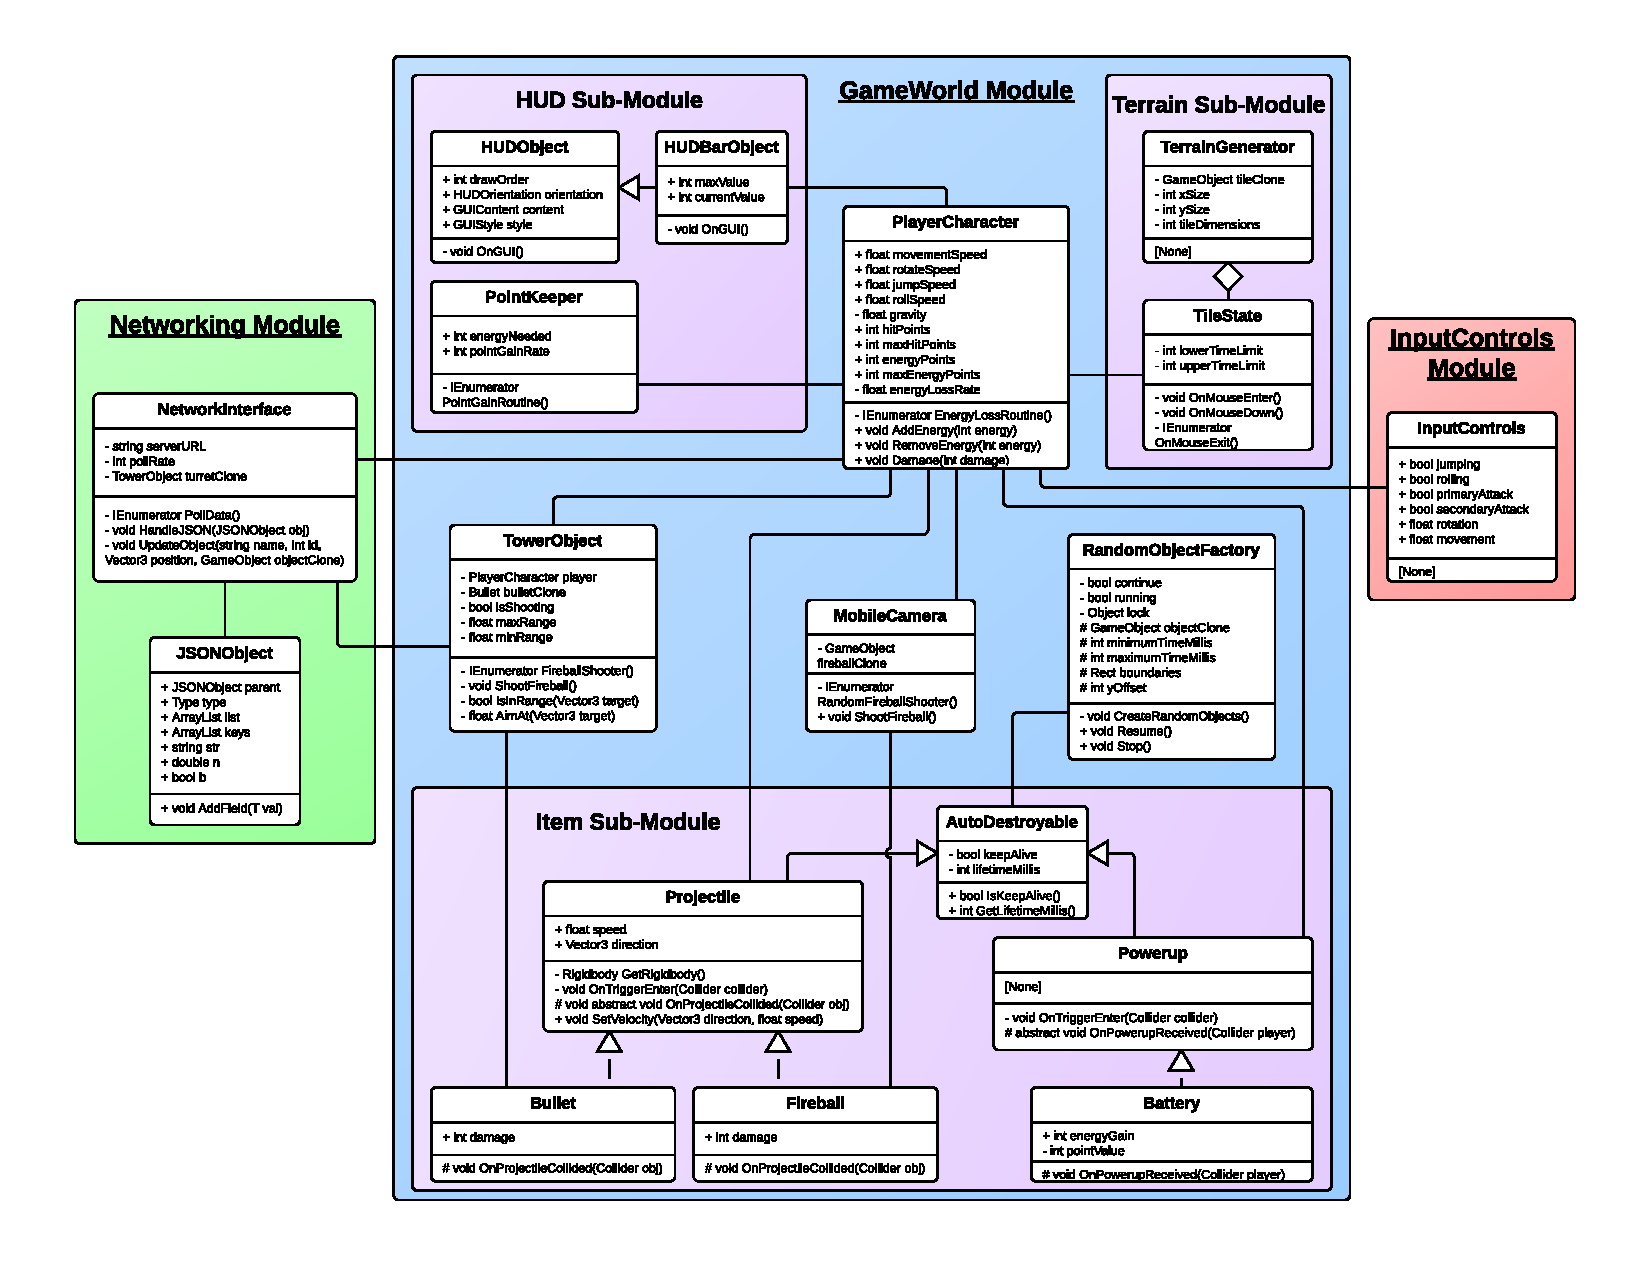
\includegraphics[scale=.75]{class}

\subsection{Code Walkthrough}
The Class diagram is admittedly complex, so let’s break it down into the most important components. The Networking module has but 2 classes. The NetworkInterface class uses the JSONObject class to exchange JSON objects with the web server. Currently, only one class actually is translated to and from a JSONObject, which is the TowerObject. We have plans to translate the PlayerCharacter into a JSONObject in the very near future.
The InputControls module is even simpler. It has one class which contains variables that are updated by the motion capture group. Every frame, the PlayerCharacter class polls the variables and moves the character accordingly.\\
The GameWorld module is by far the most complex. At the heart of the module is the PlayerCharacter class, which by necessity interacts with most other classes in the module. There are a number of other classes, for example the TowerObject class, which do something in the game to interact with the character. The TowerObject with shoot bullets at the character if it is within a certain range.\\
The GameWorld module is separated into a number of sub-modules. Each sub-module is essentially a mental delineation of types of objects in the game. The HUD sub-module contains all of the game data which appears on the heads-up display, such as the energy bar and the player’s score. It retrieves data from the PlayerCharacter about the energy level, and from Items which will be discussed shortly.\\
The Terrain sub-module is the mechanism for creating the terrain that the character moves on. The terrain in-game consists of a number of TileStates -- giant squares on the ground which can fall away after a period of time. The TerrainGenerator class creates the terrain using a number of these TileStates.\\
The Item sub-module represents the collection of objects with which the PlayerCharacter interacts. These include powerups and projectiles. The AutoDestroyable superclass provides a mechanism for automatically removing an object from the game after a certain period of time. The RandomObjectFactory sits outside of the Item sub-module but interacts closely with it. Provided a game object, this class will produce clones of that objects throughout the game scene. This is useful, for example, in spawning powerups (like batteries) randomly throughout the game world.

An important note to make is that all of the classes in the GameWorld module inherit from MonoBehavior, which is a class provided by the Unity3D game engine with hooks for performing tasks in a structured order. In particular, it provides two important functions: void Start(), which is called to initialize an object, and void Update(), which is called every frame. These two functions are what allow fluid movement in-game, yet absolute control for the programmer. Additionally, MonoBehavior inherits from GameObject, another Unity-provided class which encapsulates additional information such as mesh rendering, positions, and so forth. The net result is that the classes in the GameWorld module contain this additional information about positioning and other data, but without having to program it ourselves. All of the classes in the GameWorld module implement the two functions Start() and Update(), but to save space, these functions were not included in the class diagram.

We created a few sub-modules in order to mentally separate the tasks within the game world. It makes more sense, for example, to think of Powerups and Fireballs both as items, which behave quite similarly in most circumstances, than as two completely different entities. It simply is a grouping of objects with similar functionalities.

\section{Testing Details}

\section{Development Procedures}

Each individual worked on many aspects of the project, but for the most part, coding has been done on what was interesting to each individual. Below are the general areas of focus. In addition to these, we all shared the responsibility of writing the documentation, and communicated with each other as to what was necessary for the next demonstration session.

\subsubsection{Robin \textit{Animation and Graphics}}
In general, Robin has worked on the graphics and animation necessary for the game, most notably including the character.

\subsubsection{Etan \textit{Gameworld Tiles, Usability of Interface}}
Etan worked mainly on generating and modifying the state of the in-game tile system, as well as work on the main menu interface functionality.

\subsubsection{Nick \textit{Turrets, Minions, and Artificial Intelligence}}
The actions of the turret being able to track the player’s location and shoot the character fell under Nick’s umbrella. He also designed the minions which chase after the character and the functionality for the character to attack them.

\subsubsection{Dan \textit{Network Interface, Character Movement}}
The communication of game state information (i.e. the Network Interface module) was designed by Dan. In addition to this, he also made the character movement possible and designed the HUD and shield mechanism.

\subsubsection{Chris \textit{Main Menu Rotation, Gameworld Items}}
Chris helped provide the Main Menu with the ability to rotate between the various menus, as well as created different items for the gameworld.

\section{Reflections}

\section{Glossary and References}

\gls{Avatar}{See Character}

\gls{Blender}{An application for creating models and animations.}

\gls{Character}{The game object controlled by persons using the Kinect}

\gls{git}{A distributed version control system, which tracks and annotates changes to code.}

\gls{Github}{A hosting service for the source code of software projects.}

\gls{Kinect}{A motion capture system which gather 3D information of puppeteer's locations.}

\gls{LaTeX}{A document markup language and preparation system.}

\gls{MainDisplay}{The projector that spectators as well as puppeteers will be able to see. Will display the current state of the gameworld.}

\gls{Unity3D}{Integrated authoring tool for creating 3D video games or other interactive content such as architectural visualizations or real-time 3D animations.}

\gls{Viewport}{The view seen of the game, similar to an aerial view.}


\end{document}

